\documentclass[11pt,a4paper]{article}
\usepackage[utf8]{inputenc}
\usepackage[T1]{fontenc}
\usepackage{lmodern}
\usepackage[spanish,es-tabla]{babel}
\usepackage[margin=1.85cm]{geometry}
\usepackage[table]{xcolor}
\usepackage{array,tabularx}
\usepackage{graphicx}
\usepackage{enumitem}
\usepackage{xurl}
\usepackage[colorlinks=true,urlcolor=blue,linkcolor=black]{hyperref}
\definecolor{verde}{RGB}{0,105,65}
\definecolor{gris}{RGB}{241,244,242}
\graphicspath{{img/}{docs/img/}}
\setlength{\parindent}{0pt}
\setlength{\parskip}{5pt}
\setlength{\emergencystretch}{2em}
\renewcommand{\arraystretch}{1.16}
\setlist[itemize]{leftmargin=*,nosep}
\newcolumntype{Y}{>{\raggedright\arraybackslash}X}
\newcommand{\apartado}[1]{\par\vspace{4pt}{\large\bfseries\color{verde}#1}\par\vspace{2pt}}
\hypersetup{pdftitle={AforoSeguro: informe del desarrollo parcial},pdfauthor={Byron Daniel Loor Mendoza}}

\begin{document}
\begin{center}
{\small UNIVERSIDAD TÉCNICA ESTATAL DE QUEVEDO\\
Facultad de Ciencias de la Computación -- Carrera de Software}\par
\vspace{5pt}
{\LARGE\bfseries\color{verde} AforoSeguro}\par
{\large Informe del desarrollo parcial -- AP-U1}
\end{center}

\begin{tabularx}{\textwidth}{@{}lY@{}}
\textbf{Estudiante:} & Loor Mendoza Byron Daniel\\
\textbf{Asignatura:} & Aplicaciones Distribuidas (ISR-701), SPA 2026--2027\\
\textbf{Docente:} & Gleiston C. Guerrero-Ulloa, PhD\\
\textbf{Fecha:} & 23 de noviembre de 2026\\
\textbf{Correo:} & \texttt{bloorm2@uteq.edu.ec}
\end{tabularx}

\textbf{Repositorio:} {\small\url{https://github.com/Danxxx777/-AP-U1-Loor-Mendoza-Byron-Daniel}}\par
\textbf{Versión examinada:} código de \texttt{1822ad4}, integrado en \texttt{4b9f37a}.

\apartado{1. Alcance del prototipo}
El avance publicado permite que un coordinador lleve el contador global y que las puertas soliciten entrar, salir o consultar el estado mediante sockets TCP. La configuración fija el puerto 5000, el aforo en 10 y un token compartido. El coordinador rechaza solicitudes con formato, token o identificador de puerta incorrectos, e imprime las respuestas en consola.

\begin{tabularx}{\textwidth}{@{}p{3.5cm}Y@{}}
\rowcolor{gris}\textbf{Archivo} & \textbf{Responsabilidad implementada}\\
\texttt{Coordinador.java} & Acepta conexiones, crea un hilo por conexión y controla el contador. Incluye los modos normal e inseguro.\\
\texttt{Puerta.java} & Consola con identificador 1, 2 o 3. Envía solicitudes y muestra su respuesta; también permite probar un token incorrecto.\\
\texttt{PruebaCarga.java} & Crea 30 hilos: diez solicitudes con cada identificador de puerta. Usa una barrera para liberarlos juntos.
\end{tabularx}

Cada solicitud sigue el formato \texttt{ORDEN,token,id}. El salto de línea delimita el mensaje; \texttt{readLine()} lo recibe y \texttt{println()} lo envía. En modo normal, \texttt{synchronized (Coordinador.class)} protege la consulta y actualización del contador. En modo inseguro se omite ese bloqueo y se espera 50 ms entre leer el contador y escribir el nuevo valor.

\apartado{2. Resultado disponible de la carga}
La salida compartida por el estudiante corresponde a la prueba normal. Se transcriben sus cifras; no se presenta esta transcripción como una captura de pantalla ni como un registro Lamport.

\begin{center}
\begin{tabular}{lrrrr}
\rowcolor{gris}\textbf{Modo} & \textbf{Permitidas} & \textbf{Rechazadas} & \textbf{Errores} & \textbf{Contador}\\
Normal & 10 & 20 & 0 & 10\\
Inseguro & \multicolumn{4}{c}{Sin salida de ejecución aportada}
\end{tabular}
\end{center}

El resultado normal es coherente con el límite de 10: se autorizaron diez entradas y las veinte restantes se rechazaron. Los valores intermedios aparecen desordenados porque los hilos se ejecutan concurrentemente y el generador muestra los resultados según su lista de tareas. La comparación insegura está programada, pero sus cifras no se afirman como observadas.

\textbf{Datos de sesión aportados posteriormente:} código 1 \texttt{KD55-TB}; código 2 \texttt{662D-M6}. No estaban identificados en los mensajes del historial revisado. Su transcripción en este informe no acredita que aparecieran en los commits exigidos.

\newpage
\apartado{3. Escenarios y evidencias disponibles}
La tabla separa la evidencia disponible, las funciones del código y las partes pendientes. Las fotografías incluidas corresponden a una versión inicial de la comunicación y no demuestran la ejecución completa de los escenarios.

{\small
\begin{tabularx}{\textwidth}{@{}p{0.7cm}>{\raggedright\arraybackslash}p{3.7cm}Y@{}}
\rowcolor{gris}\textbf{E} & \textbf{Evidencia / estado} & \textbf{Interpretación y alcance}\\
E0 & Sin captura aportada de los adaptadores. & No se acredita la desconexión de la red ni la inclusión del código 1 en el primer commit.\\
E1 & Figuras 1 y 2: intercambio inicial de una solicitud y su respuesta. Parcial. & Se observa la recepción de \texttt{Estado} y la respuesta \texttt{Recibido}. No demuestra entradas por las tres puertas, una salida por P2 y el total consultado desde todas.\\
E2 & Rechazos implementados; sin evidencia completa del escenario. & El código impide superar el aforo y rechaza tokens incorrectos. Falta la captura específica de la entrada 11 y de la prueba controlada de token inválido.\\
E3 & Transcripción de la carga normal: 10/20/0 y contador 10. Parcial. & Se dispone del resultado normal. No se aportó su captura formal ni la salida de la comparación insegura.\\
E4 & No implementado en la versión publicada. & No hay latidos, temporizador de seis segundos ni registro de caída y recuperación de P3.\\
E5 & Manejo del error previsto en el cliente; sin captura específica. & \texttt{Puerta} informa que el coordinador no está disponible y que la operación no está confirmada. Esto se deduce del código, no de una ejecución documentada de E5.\\
E6 & No implementado. & No hay relojes Lamport, bitácoras por proceso ni \texttt{OrdenTotal}; por tanto, no se presentan pares causales como si se hubieran obtenido.
\end{tabularx}}

\vspace{7pt}
\begin{center}
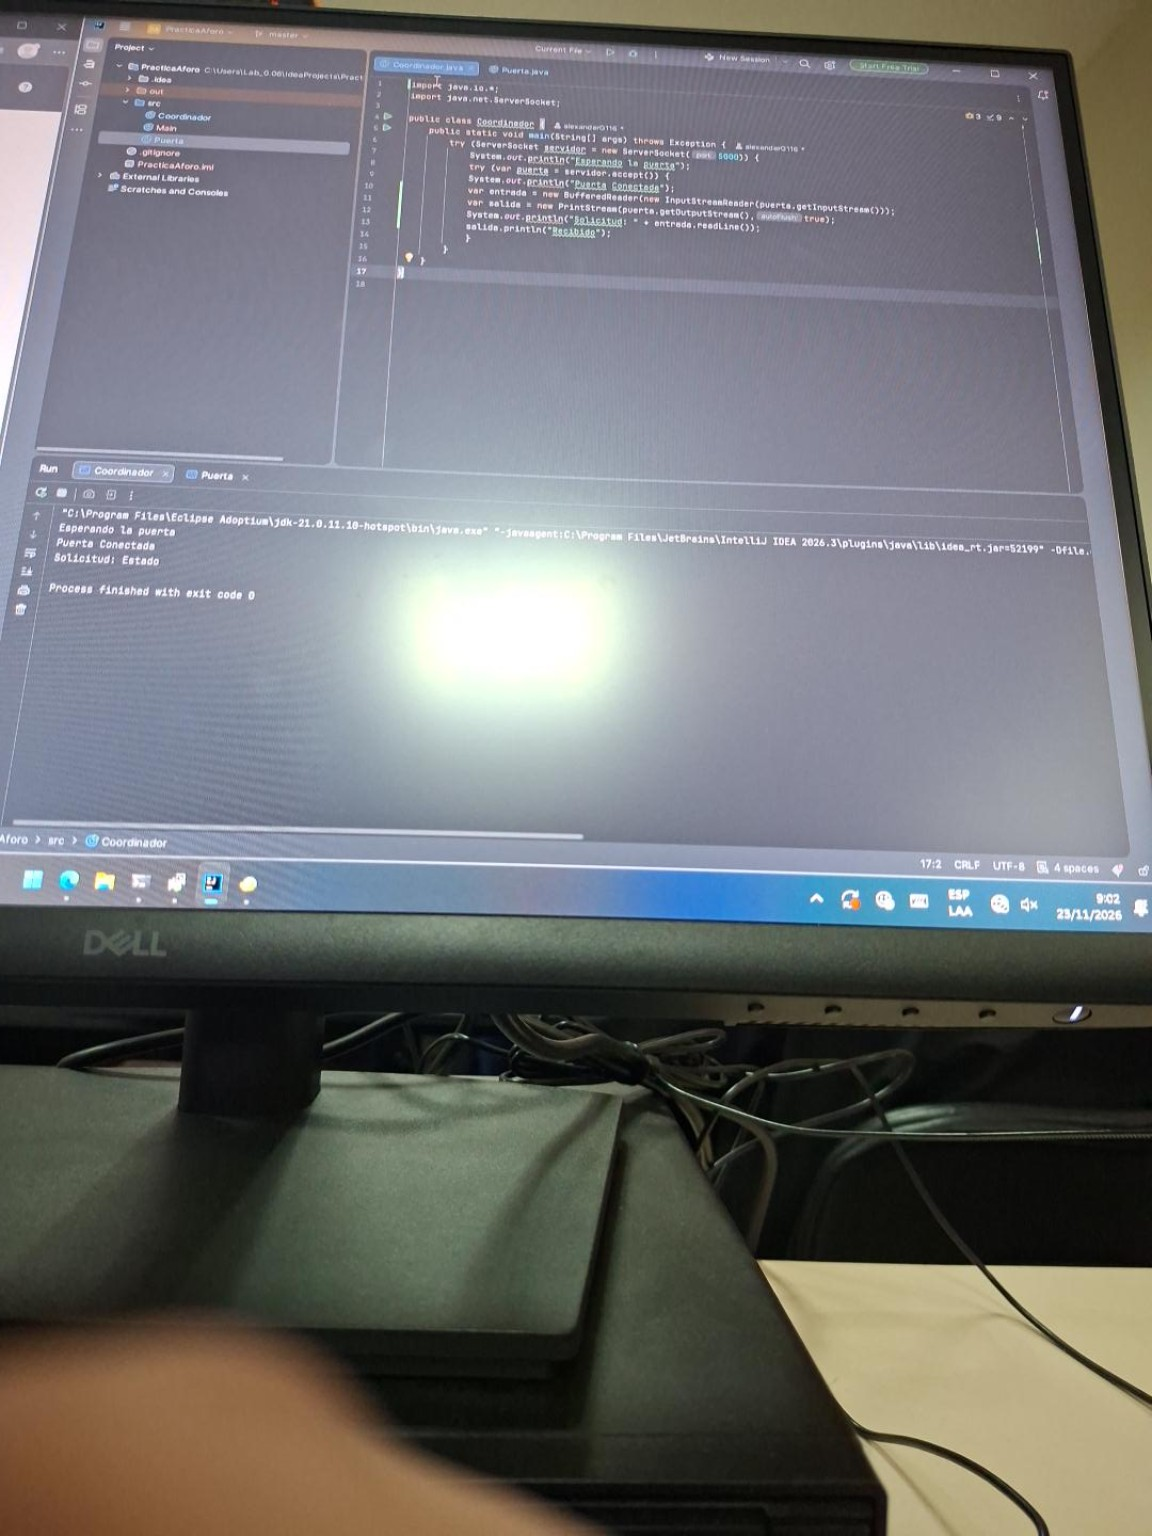
\includegraphics[width=0.94\textwidth,trim=0bp 916bp 352bp 475bp,clip]{conexion_coordinador.jpg}
\refstepcounter{figure}\par
{\small\textbf{Figura \thefigure.} Consola del coordinador: conexión y recepción de \texttt{Estado} en la versión inicial. Recorte del original conservado en \texttt{docs/img/}.}\par
\vspace{7pt}
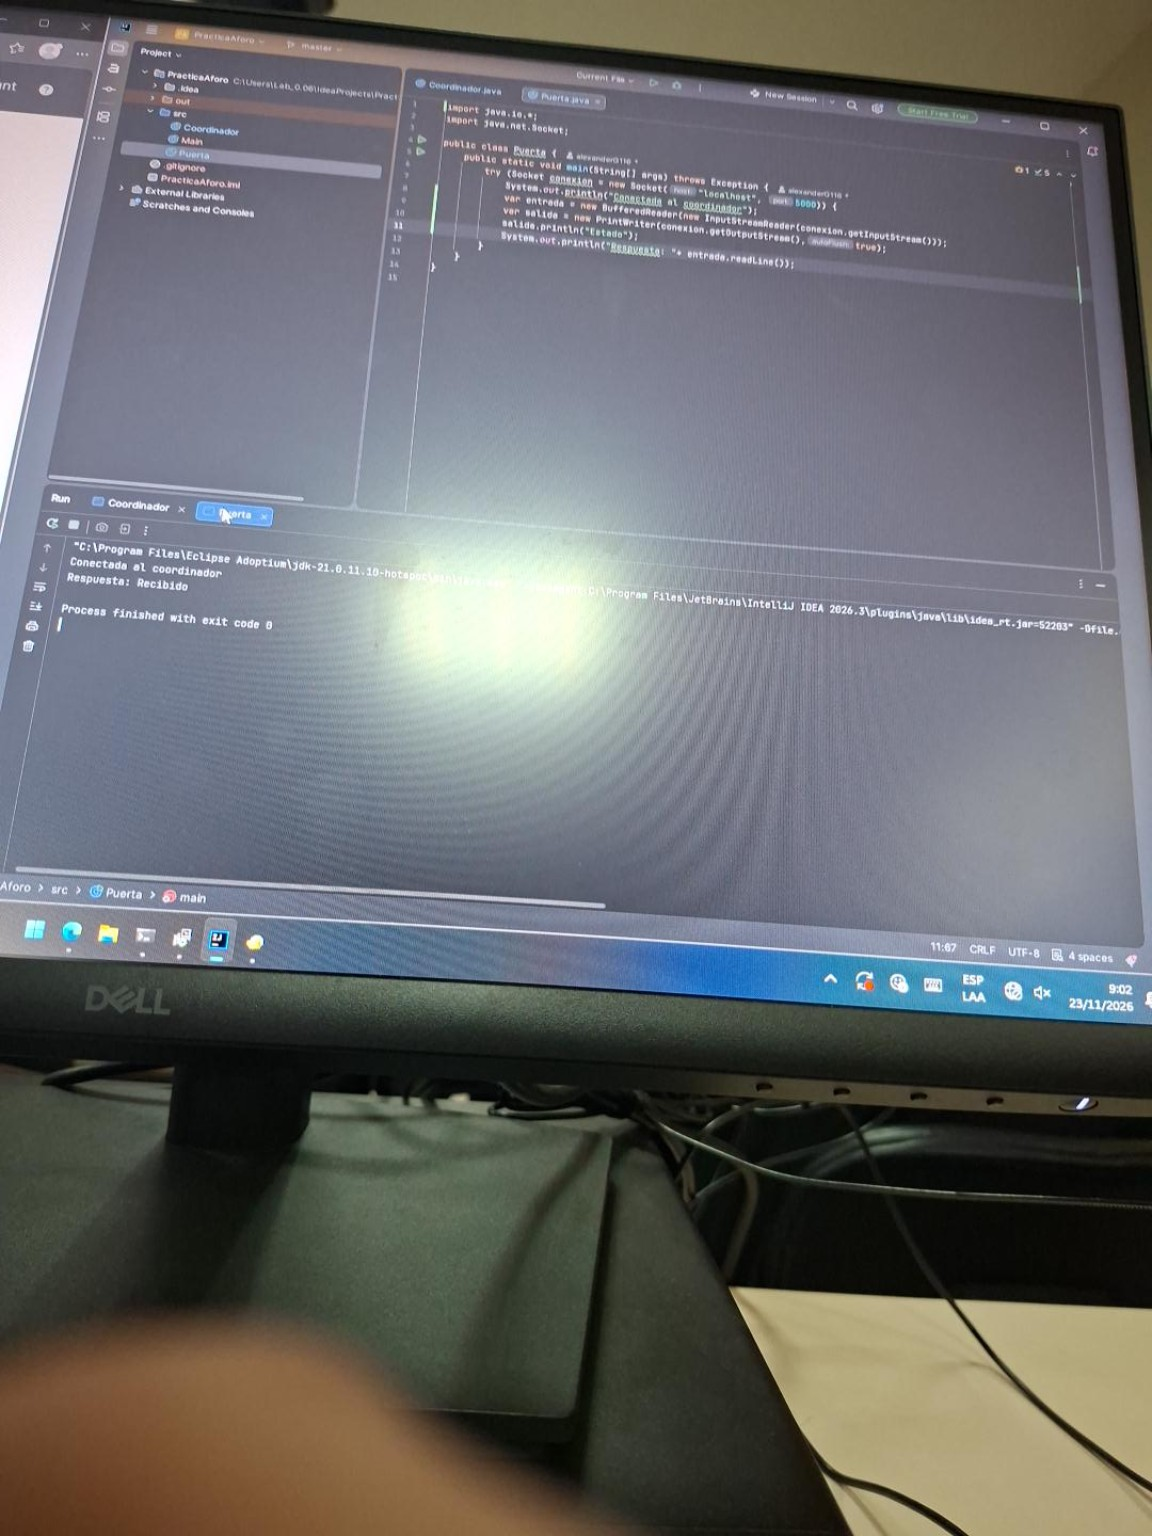
\includegraphics[width=0.94\textwidth,trim=0bp 881bp 352bp 525bp,clip]{respuesta_puerta.jpg}
\refstepcounter{figure}\par
{\small\textbf{Figura \thefigure.} Consola de la puerta: respuesta \texttt{Recibido}. Esta imagen acredita intercambio de texto, no el escenario completo de aforo.}
\end{center}

\textbf{Límite de las capturas:} los recortes facilitan la lectura de las consolas. Los originales se conservan sin modificar, pero no reúnen todos los datos de usuario, equipo y fecha requeridos para acreditar cada escenario. El archivo \texttt{carga\_normal\_transcrita.txt} identifica expresamente el origen textual de las cifras de E3.

\newpage
\apartado{4. Respuestas de análisis}

\textbf{1. E3: diferencia entre el modo normal y el inseguro.}\par
En la prueba normal se permitieron 10 entradas y se rechazaron 20. El bloqueo de \texttt{procesar()} hace que solo un hilo consulte y actualice el contador a la vez. Su costo es que las solicitudes deben esperar para entrar a esa sección. En el modo inseguro, varios hilos pueden leer el mismo valor, esperar 50 ms y escribir después el mismo incremento: pueden autorizarse más entradas de las que refleja el contador por actualizaciones perdidas. Esa posibilidad se identifica en el código; no se dispone de cifras de la ejecución insegura para compararlas con las normales.

\textbf{2. E5: consistencia, disponibilidad y CAP.}\par
La puerta requiere una respuesta del coordinador para mostrar una operación como permitida. Si la conexión falla, devuelve un error y no confirma la entrada. Por inspección del código, esta decisión privilegia el control central del aforo frente a la disponibilidad de las puertas cuando pierden comunicación. En una partición, mantener el control implica que algunas solicitudes no puedan completarse, que es el compromiso relacionado con CAP. Para el público supone esperar; para la administración, evita tratar una solicitud sin confirmación como una entrada autorizada. No se ejecutó E5 con evidencia completa. Además, un timeout no permite saber si una solicitud llegó a procesarse antes de perderse la respuesta: no hay reconciliación ni identificadores de operación.

\textbf{3. Punto único de fallo y posibles réplicas.}\par
El coordinador es el único proceso que guarda el contador. Para continuar tras su caída sería necesario replicar ese estado, detectar el fallo y elegir otro coordinador. La dificultad nueva sería mantener un contador coherente entre réplicas y evitar que dos coordinadores autoricen simultáneamente espacios que creen disponibles. El avance publicado no implementa replicación ni elección. Además, reiniciar el coordinador pone el contador en cero, por lo que no recupera el aforo previo.

\textbf{4. Falacias y tiempos de dos y seis segundos.}\par
Los intervalos de latido de 2 s y detección de 6 s pertenecen al planteamiento, pero no se implementaron en este avance. Su elección debe considerar que la red no es instantánea y puede fallar: un retraso no demuestra que un proceso haya muerto. Con una latencia de 7 s, un detector con umbral de 6 s podría sospechar una caída aunque la puerta siguiera activa. En el código publicado, el cliente también podría agotar su espera de lectura de 5 s antes de recibir una respuesta tan demorada.

\apartado{5. Limitaciones y trazabilidad}
El desarrollo quedó concentrado en comunicación, autenticación y control concurrente del aforo. Los mensajes y rechazos se muestran en consola; no se guardan como bitácoras persistentes. No se implementaron las partes C y D: latidos, estados de actividad, relojes lógicos y orden total. La prueba de carga representa los identificadores P1, P2 y P3 mediante hilos; no inicia tres procesos de puerta por sí misma.

El historial previo a este documento tiene seis commits, cuatro de ellos con cambios de código. El primer commit local de código, \texttt{02e2683}, conserva la identidad que estaba configurada en el equipo del laboratorio; los posteriores contienen los datos del estudiante. Este informe se incorpora después del desarrollo y conserva esas fechas y mensajes. No sustituye las evidencias temporales, de autoría y de ejecución exigidas en la actividad.

\textbf{Uso de IA:} la implementación y la elaboración de este informe contaron con asistencia de IA generativa. Esta declaración deja constancia de su uso; no acredita cumplimiento de la condición de trabajo sin IA establecida en el planteamiento.

\end{document}
